\chapter{L4 and L5:  Quotients, Remainders, and Modular Congruence }

\section{L4:  The Quotient-Remainder Theorem}

You have hopefully become an expert at proving basic statements about parity and divisibility.  You may have been very tempted to use the concept of a \textbf{remainder} when making these kinds of arguments.  Unfortunately we have not, as yet, defined what a remainder is!  We rectify that situation in this chapter.

\begin{xca}
		Compute $953 \div 7$ as you would in elementary school to obtain a quotient and a remainder, without worrying about the precise definitions of the words ``quotient'' and ``remainder''.
	\end{xca}

\begin{solutions}
    \intlongdivision{953}{7}
    
    So $953 = 136 \cdot 7 + 1$.
    
    We say that the dividend is $953$, the divisor is $7$, the quotient is $136$ and the remainder is $1$.
    
    Notice that this usage of the term ``divisor'' is in conflict with our definition of this word!  Here (and in elementary school) it is used to just mean ``the number we are dividing by''.  It is an unfortunate reality that, even in mathematics, we sometimes have more than one meaning for a given word.  In these situations we just need to understand, from context, which meaning is intended. 
	\end{solutions}

Let us attempt to craft some definitions which we will be satisfied with.

If $n \in \mathbb{Z}$ is a dividend and $d$ is a divisor then we want to obtain a quotient $q$ and a remainder $r$.  By analogy with $953 = 136 \cdot 7 + 1$ we will want

\[
n = dq + r
\]

However, this condition is not sufficient to uniquely specify which $q$ and $r$ we are talking about!

For instance it is also true that $953 = 135 \cdot 7 + 8$ (we just ``took out one seven'').  We would not call $135$ the quotient and $8$ the remainder because $8$ is larger than $7$.   We want our remainder $r$ to satisfy $0 \leq r < d$.

So say that $n \in \mathbb{Z}$ and $d \in \mathbb{Z}^+$.  Assume that we have found integers $q_1$, $r_1$, $q_2$, and $r_2$ with

\begin{align*}
n &= q_1d + r_1 \textrm{ with $0 \leq r_1 < d$}\\
n &= q_2d + r_2 \textrm{ with $0 \leq r_2 < d$}
\end{align*}

Can we conclude that $q_1 = q_2$ and $r_1 = r_2$?  In other words, does the condition that 

\[
n = qd + r \textrm{ with $0 \leq r < d$}
\]

\textbf{uniquely} specify $q$ and $r$?

We can argue that $q_1 = q_2$ and $r_1 = r_2$ as follows:

\begin{fitch}
	\textrm{Let $n \in \mathbb{Z}$ be arbitrarily chosen.}\\
	\textrm{Let $d \in \mathbb{Z}^+$ be arbitrarily chosen.}\\
	\textrm{Let $q_1,q_2,r_1,r_2 \in \mathbb{Z}$ be chosen arbitrarily.}\\
	\textrm{Assume $n  = q_1d+r_1$ and $n = q_1d + r_2$ and $0 \leq r_1 < d$ and $0 \leq r_2 < d$}\\
	\fa  q_1d + r_1 = q_2d + r_2\\
	\fa (q_1-q_2)d = r_2 - r_1\\
	\fa |q_1 - q_2|d = |r_2 - r_1|\\
	\fa 0 \leq |r_2 - r_1| < d \textrm{ since $0 \leq r_1 < d$ and $0 \leq r_2 < d$}\\
	\fa \textrm{Assume $|r_2- r_1| \neq 0 $}\\
	\fa \fa \textrm{Then $|q_1 - q_2|d \neq 0$, so $|q_1 - q_2| \neq 0$}\\
	\fa \fa \textrm{Then $|q_1 - q_2|d  \geq d$ since $|q_1 - q_2|$ is at least $1$}\\
	\fa \fa \textrm{This is absurd:  we cannot have $|q_1 - q_2|d = |r_2 - r_1|$ when $|q_1 - q_2|d \geq d$ and $|r_2 - r_1| < d$}\\
	\fa \textrm{So $|r_2 - r_1| = 0$, which implies $r_2 = r_1$}\\
	\fa \textrm{So $(q_1 - q_2)d = 0$, which implies $q_2 = q_1$}\\
	\end{fitch}


We have justified that \textbf{if} we can find integers $q$ and $r$ so that $n = dq + r$ with $0 \leq r < d$, \textbf{then} this pair of integers is the \textbf{unique} pair which works.

We have not yet justified that it is always possible to find such a pair of integers.  The proof of this relies on something called the ``principle of mathematical induction'' which we will learn later.  So we will skip the proof for now and come back to it when we discuss mathematical induction.

Until then I ask you to (conditionally) believe the following theorem:

\begin{theorem}[Quotient-Remainder Theorem]
Let $n$ be any integer and $d$ be any positive integer. Then there are unique integers $q$ and $r$ satisfying

\[
n = qd + r \textrm{ with  $0 \leq r < d$}
\]

We call $q$ the \index{quotient} \textbf{quotient} and $r$ the \index{remainder} \textbf{remainder}.
\end{theorem}

In the programming language Python  $n/d$ will output the quotient and $n\% d$ will output the remainder.  I recommend using the following website as a calculator using these commands.  Just enter an expression (like $953/7$ or $953 \% 7$) and click ``run'':

\begin{center}
\url{http://pythonfiddle.com/}
\end{center}

Although this is not typically done in mathematics, we will also adopt these quotient and remainder \textbf{operations} in this text.

\begin{definition}
		Let $n \in \mathbb{Z}$ and $d \in \mathbb{Z}^+$.  We define $n/d  = q$ and $n \% d = r$ where $q$ and $r$ are the quotient and remainder ensured by the QR theorem.
	\end{definition}

\begin{xca}
	Calculate the quotients and remainders in each of the following situations by hand.  Then double check yourself using Python.
	\begin{enumerate}
			\item $22/4$ and $22\%4$
			\item $(-22)/4$ and $(-22)\% 4$
			\item $11/1$ and $11\%1$
			\item $11/2$, $11\%2$.
			\item $0/5$, $0\%5$.
			\item $(-452)/6$, $(-452) \% 6$.
		\end{enumerate}
	\end{xca}

\begin{solutions}
	\begin{enumerate}
		\item I can see ``immediately'' that $22 = 5(4) + 2$, so the quotient is $5$ and the remainder is $2$.
		\item This is a little tougher.  My first thought was to try to use $-5(4) =-20$, but then I realized adding a positive number to this will never give me $-22$.  So I went ``one 4 further in the negative direction" to obtain $-6(4) = -24$.  Now I see that I can add $2$ to get $-22$.
		
		Since $-22 = (-6)(4) + 2$ we have that the quotient is $-6$ and the remainder is $2$.
		\item It is clear that $11 = 11(1) + 0$, so the quotient is $11$ and the remainder is $0$.
		\item I can see that $11 = 5(2)+ 1$ so the quotient is $5$ and the remainder is $1$.  Hmm, this looks a lot like the kind of calculation I do to confirm that $11$ is odd...
		\item $0 = 0(5) + 0$ so both the quotient and remainder are $0$.
		\item Generalizing from the second problem I do long division:
		
    \intlongdivision{452}{6}
    
    So $75(6)+2= 452$, which means $75(6) = 450$, and so $(-75)(6) = -450$.  This is ``not negative enough'', so I go ``one six further'' to get $(-76)(6) = -456$.  Finally I see that I can add $4$:
    
    $-452 = (-76)(6) + 4$
    
    So the quotient is $-76$ and the remainder is $4$.
    \end{enumerate}
	\end{solutions}


We can use quotients and remainders to establish an equivalent condition for divisibility statements.

\begin{theorem}
		Let $n \in \mathbb{Z}$ and $d \in \mathbb{Z}^+$.  Then $d \divides n$ if and only if $n \% d = 0$.
	\end{theorem}

		\begin{fitch}
				\textrm{Let $n \in \mathbb{Z}$ and $d \in \mathbb{Z}^+$ be chosen arbitrarily} & $\forall$-intro\\
				\textrm{Assume $d \divides n$} & $\implies$ -intro\\
				\fa \textrm{Then there is an integer $k$ with $n = dk$}\\
				\fa \textrm{Then $n = dk + 0$}\\
				\fa \textrm{So $n \% d = 0$}\\
				\textrm{So $d \divides n$ implies $n \% d = 0$} & $\implies$- intro, (2)\\
				\textrm{Assume $ n \% d = 0$} & $\implies$-intro\\
				\fa \textrm{Then there exists an integer $k$ with $n  = kd + 0 $}\\
				\fa \textrm{So $d \divides n$}\\
				\textrm{So  $n \% d = 0$  implies $d \divides n$} & $\implies$- intro, (7)\\
				\textrm{So $n \% d = 0 \bi d \divides n$} & $\bi$-intro, (6), (10)\\
				\textrm{So $\forall n \in \Z: \forall d \in \Z^+: n \% d = 0 \bi d \divides n$} & $\forall$-intro, (1)
			\end{fitch}
		
\begin{theorem}
		For all $n \in \Z$, $n$ is even if and only if $n\%2 = 0$ and $n$ is odd if and only if $n\%2 = 1$.
	\end{theorem}

I encourage you to prove this theorem yourself!  It is very similar to the proof above.

The following theorem appears innocuous, but we actually need the QR theorem  to prove it!

\begin{theorem}
		Every integer is either even or odd.
	\end{theorem}

\begin{proof}
	
	More formally we are trying to show that
	
	\[
	\forall n \in \mathbb{Z}: \textrm{$n$ is even} \vee \textrm{$n$ is odd}
	\]
	
	We will follow the proof outline, but we will use the QR theorem to introduce a case analysis on the remainder after division by $2$.
	
	\begin{fitch}
			\textrm{Let $n \in \mathbb{Z}$ be chosen arbitrarily.} & $\forall$-intro\\
			\textrm{By the QR theorem we know $n\%2 = 0$ or $n\%2 = 1$}\\
			\textrm{Case 1:  Assume $n\%2 = 0$} & $\vee$-elim (2)\\
			\fa \textrm{Then $n$ is even}\\
			\fa \textrm{So ($n$ is even) $\vee$ ($n$ is odd)} & $\vee$-intro (4) \\
			\textrm{Case 2:  Assume $n\%2 = 1$} & $\vee$-elim (2)\\
			\fa \textrm{Then $n$ is odd}\\
			\fa \textrm{So ($n$ is even) $\vee$ ($n$ is odd) } & $\vee$-intro (7) \\
			\textrm{So ($n$ is even) $\vee$ ($n$ is odd) } & $\vee$-elim (2), (3), (6)\\
			\textrm{So } \forall n \in \mathbb{Z}: \textrm{$n$ is even} \vee \textrm{$n$ is odd} & $\forall$-intro (1)
		\end{fitch}
	
	\end{proof}

\begin{xca}
	Prove that  $n^2 - 3$ is never divisible by $5$ for any integer $n$
	
	Hint:  In your proof use QR to write $n \%5 = r$ with $r = 0,1,2,3,4$ and do a case analysis.
	\end{xca}

\newpage
				
				\begin{fitch}
					\ftag{~} \textrm{\underline{To prove:  $\forall n \in \mathbb{Z}: \neg( 5 \divides (n^2 - 3))$}}\\
						\textrm{Let $n \in \mathbb{Z}$ be chosen arbitrarily} & $\forall$-intro\\
						\textrm{Assume $5 \divides (n^2 - 3)$} & $\neg$-intro\\
						\fa \textrm{So there is an integer $k$ with $n^2 - 3 =5k$}\\
						\fa \textrm{So $n^2 \% 5 = 3$}
						\fa \textrm{By QR, $n \% 5 = r$ with $r= 0 , 1, 2,3$ or $4$}\\
						\fa \textrm{Case 1:  $r=0$} & $\vee$-intro\\
						\fa \fa \textrm{Then $n = 5q$}\\
						\fa \fa \textrm{So $n^2 \% 5 = (25q^2) \% 5 = 0$}\\
						\fa \fa \bot\\
						\fa \textrm{Case 2:  $r = 1$} & $\vee$-intro\\
						\fa \fa \textrm{Then $n = 5q + 1$}\\
						\fa \fa \textrm{So $n^2 = 25q^2 + 10q + 1$}\\
						\fa \fa \textrm{So $n^2\% 5 = 1$}\\
						\fa \fa \bot\\
						\fa \textrm{Case 3:  $r = 2$} & $\vee$-intro\\
						\fa \fa \textrm{Then $n = 5q + 2$}\\
						\fa \fa \textrm{So $n^2 = 25q^2 + 20q + 4$}\\
						\fa \fa \textrm{So $n^2 \% 5 = 4$}\\
						\fa \fa \bot\\
						\fa \textrm{Case 4:  $r = 3$} & $\vee$-intro\\
						\fa \fa \textrm{Then $n = 5q + 3$}\\
						\fa \fa \textrm{So $n^2 = 25q^2 + 30q + 5 + 4$}\\
						\fa \fa \textrm{So $n^2 \% 5 = 4$}\\
						\fa \fa \bot\\
						\fa \textrm{Case 5:  $r = 4$} & $\vee$-intro\\
						\fa \fa \textrm{Then $n = 5q + 4$}\\
						\fa \fa \textrm{So $n^2 = 25q^2 + 40q + 15 + 1$}\\
						\fa \fa \textrm{So $n^2 \% 5 = 1$}\\
						\fa \fa \bot\\
						\fa \textrm{In all cases we proved $\bot$} & $\vee$-intro lines 5, 9, 14, 19, 24\\
						\textrm{So $\neg( 5 \divides n^2 - 3)$} & $\neg$-intro, line 2\\
						\textrm{So $\forall n \in \mathbb{Z}: \neg( 5 \divides (n^2 - 3))$} & $\forall$-intro, line 1.
					\end{fitch}

\newpage

\section{L4: Homework}

\begin{xca}
	Compute each of the following by hand:
	\begin{enumerate}
		\item $44/3$
		\item $44\%3$
		\item $(-72)/5$
		\item $(-72)\%10$
		\item $11/1$
		\item $11 \%1$
		\end{enumerate}
	\end{xca}

\begin{xca}
Prove each of the following statements.  You may assume that the Quotient Remainder theorem is true.
	\begin{enumerate}
		\item If $x\%5 = 3$ and $y \%5 = 2$ then $xy \% 5 = 1$.
		\item For every integer $x$, $x^2 + x$ is even.
		\item For every integer $x$, $x(x+1)(x+2)$ is divisible by $3$.
		\item If $9 \divides x^2$ then $3 \divides x$.
	\end{enumerate}
\end{xca}
				
\section{L5: Modular Congruence}

In the last section we proved the theorem that $n^2 - 3$ is never divisible by $5$ for any integer $n$.  The proof boiled down to a case analysis on the value of $n \% 5$.  So, for the purposes of this argument, the exact value of $n$ ``didn't really matter'':  the thing that mattered was the remainder of $n$ upon division by $5$.  Since the numbers $..., -7, -2, 3, 8, 13, 18, 23, ...$  all  have a remainder of $3$ when divided by $5$, they would all be treated in the same way by the argument we gave.  In fact, we established in Case 2 of that proof that all of these numbers would have the property that if $n\%5 = 3$ then it follows that $n^2 \% 4$.

We will attempt to capture these ideas in the following definition of \textbf{modular congruence}, which is a kind of ``relaxed'' notion of equality where we consider two integers to be ``the same'' (or congruent) if they generate the same remainder when divided by some ``modulus''.

Notice that in the list $..., -7, -2, 3, 8, 13, 18, 23, ...$, the difference between any two elements is a multiple of $5$.  For instance $18-3 = 15$ and $23 - (-2) = 25$.  It makes sense that if the difference of two numbers is a multiple of $5$, then the two numbers will have the same remainder when divided by $5$.  This motivates the following definition:

\begin{definition}
		Let $m \in \Z$.  Let $a,b\in \Z$.  We will say that $a$ is congruent to $b$ modulo $m$ if  $m \divides (b-a)$.	 In this case we write $a \equiv b \mod m$.
\end{definition}

The following picture might help you to understand the definition.  

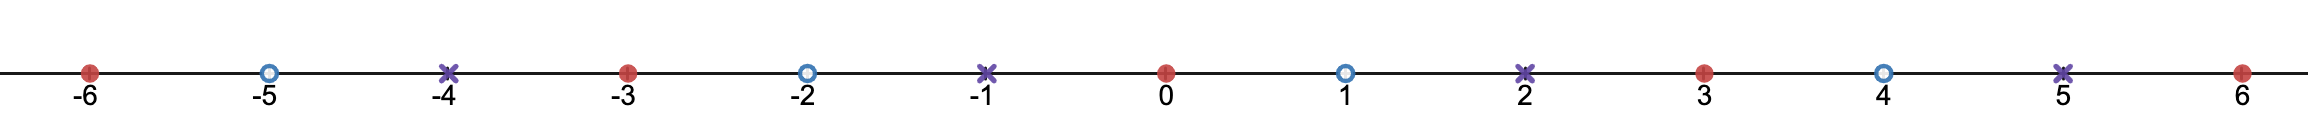
\includegraphics[scale=0.35]{mod3}

All of the numbers with the same shape are equivalent modulo $3$.  For instance, the distance from $-2$ to $4$ is $6$, which is a multiple of $3$, so $-2$ and $-4$ are equivalent modulo $3$.  For that reason they are both given blue hollow circles in this picture.
 
\begin{theorem}
Let $m$ be a positive integer.  Then $a \equiv b \mod m$ if and only if $a \% m = b \% m$.  In other words, for positive modulus $m$, two numbers are congruent modulo $m$ if and only if they have the same remainder upon division by $m$.  
\end{theorem}

\begin{fitch}
		\textrm{Let $a,b \in Z^+$, $m \in \Z^+$ be chosen arbitrarily} & $\forall$-intro\\
		\textrm{Assume  $a \equiv b \mod m$} & $\implies$-intro\\
		\fa \textrm{Then $m \divides (b-a)$}\\
		\fa \textrm{Choose a $k \in \Z^+$ with $b - a = mk$}\\
		\fa \textrm{Let $a/m = q_a$, $a \% m = r_a$, $b/m = q_b$, $b \% m = r_b$}\\
		\fa \textrm{Assume, without loss of generality, that $r_b \geq r_a$}\\
		\fa \textrm{$a = q_am+r_a$ and $b = q_bm+r_b$}\\
		\fa \textrm{$b-a = (q_b - q_a)m  + (r_b - r_a)$}\\
		\fa \textrm{$mk = (q_b - q_a)m  + (r_b - r_a)$}\\
		\fa \textrm{Since $0 \leq r_b - r_a< m$ and $m \divides(r_b - r_a)$, $r_b - r_a = 0$}\\
		\fa r_b = r_a\\
		\fa a \% m =  b \% m\\
		 a \equiv b \mod m \implies  a \% m =  b \% m & $\implies$-intro (2)\\
		\textrm{Assume $a \% m =  b \% m = r$ }  & $\implies$-intro\\
		\fa \textrm{Then $a = q_am + r$ and $b = q_bm + r$}\\
		\fa \textrm{So $b - a = (q_b - q_a)m$}\\
		\fa \textrm{So $m \divides (b-a)$}\\
		\fa \textrm{So $a \equiv b \mod m$}\\
		a \% m =  b \% m \implies a \equiv b \mod m & $\implies$-intro (14)\\
		a \% m =  b \% m \bi a \equiv b \mod m & $\bi$-intro (13), (19)\\
		\forall a,b \in \Z^+: \forall m \in \Z^+:  a \equiv b \mod m \bi a \% m =  b \% m & $\forall$-intro (1)
	\end{fitch}


I leave the proof of the following theorem to the reader.\footnote{It is \textbf{very} important that you actually prove these statements!}
\begin{theorem}
		The following basic properties of modular congruence are all true:
		
		\begin{enumerate}
			\item (Reflexivity) $a \equiv a \mod N$ for all integers $a$.
			\item (Symmetry) If $a \equiv b \mod N$ then $b \equiv a \mod N$.
			\item (Transitivity) If $a \equiv b \mod N$ and $b \equiv c \mod N$ then $a \equiv c \mod N$.
			\item (Respects addition) If $a \equiv a' \mod N$ and $b \equiv b' \mod N$ then $a+b \equiv a'+b' \mod N$.
			\item (Respects multiplication)If $a \equiv a' \mod N$ and $b \equiv b' \mod N$ then $ab \equiv a'b' \mod N$.
		\end{enumerate}
	\end{theorem}

These properties allow us to calculate remainders with surprising speed and agility, and far more efficiently that we could by using long division:

\begin{xca}
	Calculate $(73^3 + 5^9) \% 3$
	\end{xca}

\begin{solutions}
	\begin{align*}
		73^3 + 5^9 \equiv 1^3 + 2^9 \mod 3\\
		\equiv 1 + 2(2^8) \mod 3\\
		\equiv 1+2(4^4) \mod 3\\
		\equiv 1+2(1^4)\mod 3\\
		\equiv 3 \mod 3\\
		\equiv 0 \mod 3
		\end{align*}
	
Imagine how hard it would have been to calculate $73^3 + 5^9$ and then find the quotient and remainder after division by $3$!
	\end{solutions}


\section{L5: Homework}

\begin{xca}
		Use modular arithmetic to compute each of the following by hand.
	\begin{enumerate}
			\item $17^{43} + 18^{15} \% 7$
			\item $23^{12} \% 5$
			\item $23^{12} \% 10$
			\item $23^{12} \% 100$
			\item Compute the last digit of $17^{20}$.
		\end{enumerate}
	\end{xca}

\begin{xca}
		Prove each of the following statements.
		
		\begin{enumerate}
				\item (Reflexivity) $a \equiv a \mod N$ for all integers $a$.
				\item (Symmetry) If $a \equiv b \mod N$ then $b \equiv a \mod N$.
				\item (Transitivity) If $a \equiv b \mod N$ and $b \equiv c \mod N$ then $a \equiv c \mod N$.
				\item (Respects addition) If $a \equiv a' \mod N$ and $b \equiv b' \mod N$ then $a+b \equiv a'+b' \mod N$.
				\item (Respects multiplication)If $a \equiv a' \mod N$ and $b \equiv b' \mod N$ then $ab \equiv a'b' \mod N$.
			\end{enumerate}
	\end{xca}

\begin{xca}
	Prove each of the following statements.
	
	\begin{enumerate}
			\item If $a \cong b \mod n$  and $m \divides n$ then $a \cong b \mod m$.
			\item $6^n - 1$ is divisible by $5$ for all natural numbers $n$.
			\item For every $n \in \Z$ if $n \cong 3 \mod 7$ there is an $m$ in $\Z$ with $nm \cong 2 \mod 7$.
			\item If $n^2$ is congruent to $1$ mod $7$ then $n$ is either congruent to $1$ or $6$ mod $7$.  
			\item (hard) $n \cong 1 \mod 2$ if and only if $n^2 \cong 1 \mod 8$.
	\end{enumerate}
\end{xca}







